\subsection{Motivation \& Background}

\begin{figure}
\centering
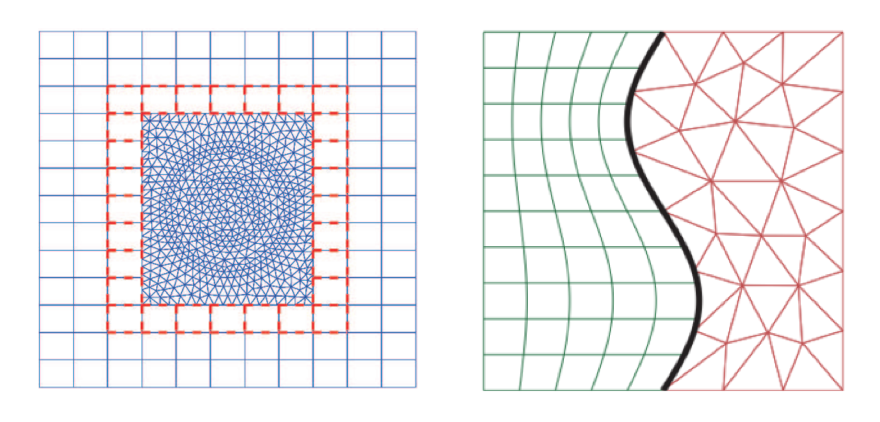
\includegraphics[width=0.8\linewidth,trim=4 4 4 4,clip]{figures/nonconforming_samples.png}
\caption{Two examples demonstrating use of nonconforming interfaces. Left: Zhu, Chen, Zhong, and Liu \cite{zhu2011hybrid}.
	 Right: Kozdon and Wilcox \cite{kozdon2016stable}}
\label{fig:nonconforming_samples}
\end{figure}

\subsubsection{Goals, Bounds, and Impact}

This section of the proposal targets a lack of high-order accurate and
provably stable interface conditions between structured and unstructured
meshes for computational fluid dynamic simulations. In particular, our aim
is to create a provably stable and accurate interface between summation-by-parts
finite difference discretizations (structured) and discontinuous Galerkin
methods (unstructured).  Achieving this would provide an option to create localized
areas of unstructured meshing (with superior flexibility for discretizing complex
boundaries/geometries) in existing simulations, providing an alternative to
overset curvilinear meshes.

%===========================================================================
\subsection{Governing Equations}

The initial problem for which our new hybrid method will be targeted is
the acoustic wave equation in two dimensions, in first-order form:
\begin{align}
&\rho \frac{\partial v_{i}}{\partial t} + \frac{\partial p}{\partial x_{i}} = 0 \hspace{2mm} (i = 1, 2), \\
&\frac{\partial p}{\partial t} + \lambda \left(\frac{\partial v_{1}}{\partial x_{1}} + \frac{\partial v_{2}}{\partial x_{2}} \right) = 0
\end{align}

As in \cite{kozdon2016stable}, our aim will be to prove the semi-discrete hybrid discretization
stable by proving that
\begin{align}
\frac{d\mathcal{E}}{dt} \leq 0
\end{align}
where the total energy of the semi-discrete system $\mathcal{E}$ is obtained by summing the
energy $E$ of each discretization block:
\begin{align}
\mathcal{E} = \sum_{blocks} E
\end{align}

%===========================================================================
\subsection{Numerical Methods}

\subsubsection{Summation-by-Parts Operators}

For the structured discretization that makes up one component of the proposed hybrid, we make use of several
finite difference operators that possess the summation-by-parts (SBP) property. Taking two matrices
${P,Q}$, we here state that these two matrices are SBP matrices of order $p$ provided 
\begin{itemize}
\item $P^{-1}Q\mathbf{v}$ is an order $h^{p}$ approximation to $\partial/\partial x$, where $h$ is the spatial step size in one dimension.
\item P is a symmetric positive-definite matrix.
\item $Q + Q^{T} = \text{diag}(-1,0,0,...,0,1)$.
\end{itemize}
These conditions together ensure that the discrete version of the integration by parts property holds; that is,
\[\langle P^{-1}Q\mathbf{x},\mathbf{y}\rangle_{P} = \mathbf{x}_{N}\mathbf{y}_{N} -  \mathbf{x}_{1}\mathbf{y}_{1} - \langle \mathbf{x},P^{-1}Q\mathbf{y}\rangle _{P}. \]

The resulting operators can be either explicit (in this case, $P$ is purely diagonal) or implicit.
This theory, originally presented in \cite{strand1994summation}, can also be extended to higher
dimensions using Kronecker products.  For example, in two dimensions, the matrices $H^{-1} G_x$
and $H^{-1} G_y$ define the $x$- and $y$- derivatives on a two-dimensional grid:
\begin{align}
H = P_{x} \otimes P_{y} \notag \\
G_{x} = Q_{x} \otimes P_{y} \notag \\
G_{y} = P_{x} \otimes Q_{y} \notag
\end{align}
Note that this formulation assumes that we have ${P_{x},Q_{x}}$, a pair of $n_{x} \times n_{x}$ SBP
matrices of approximation order $p$, and ${P_{y},Q_{y}}$, a pair of $n_{y} \times n_{y}$ SBP matrices
of approximation order $q$. Finally, we also note that these SBP operators do not guarantee strict
stability for an initial boundary value problem. We must also apply the boundary conditions using a
formulation that permits an energy estimate. More information on these boundary conditions, called
simultaneous approximation term (SAT) boundary conditions, can be found at \cite{svard2007stable},
\cite{svard2008stable}, and \cite{bodony2010accuracy}.

More information on SBP operators of various order, including the coefficients themselves, can be found
in \cite{strand1994summation}, \cite{carpenter1993time}, \cite{mattsson2004stable}. For this work,
we will employ diagonal-norm SBP operators for the finite difference discretizations.

\subsubsection{Discontinuous Galerkin Method}

\subsubsection{Interface Method}

%===========================================================================
\subsection{Validation}

The test problem for validation will match that of \cite{kozdon2016stable},
modeling the two-dimensional acoustic wave equation in first-order form with
the following initial condition:
\begin{align}
  p(x_{1},x_{2},0) &=
  \cos\left(k_{1} x_{1}\right)\cos\left(k_{1} x_{2}\right)
  +
  \sin\left(k_{2} x_{1}\right)\sin\left(k_{2} x_{2}\right),\\
  v_{i}(x_{1},x_{2},0) &= 0,~ \quad i=1,2,
\end{align}
where $k_{1} = \pi/2$ and $k_{2} = \pi$. All exterior boundary conditions are
zero pressure (free-surface) conditions. The exact solution of this problem is
\begin{align}
  p(x_{1},x_{2},t) &=
  \cos\left(\omega_{1} t\right)
  \cos\left(k_{1} x_{1}\right)\cos\left(k_{1} x_{2}\right)
  +
  \cos\left(\omega_{2} t\right)
  \sin\left(k_{2} x_{1}\right)\sin\left(k_{2} x_{2}\right),\\
  v_{1}(x_{1},x_{2},t) &=
  \frac{k_{1}}{\omega_{1}} \sin\left(\omega_{1} t\right)
  \sin\left(k_{1} x_{1}\right)\cos\left(k_{1} x_{2}\right)
  -
  \frac{k_{2}}{\omega_{2}} \sin\left(\omega_{2} t\right)
  \cos\left(k_{2} x_{1}\right)\sin\left(k_{2} x_{2}\right),\\
  v_{2}(x_{1},x_{2},t) &=
  \frac{k_{1}}{\omega_{1}} \sin\left(\omega_{1} t\right)
  \cos\left(k_{1} x_{1}\right)\sin\left(k_{1} x_{2}\right)
  -
  \frac{k_{2}}{\omega_{2}} \sin\left(\omega_{2} t\right)
  \sin\left(k_{2} x_{1}\right)\cos\left(k_{2} x_{2}\right),
\end{align}
where $\omega_{j} = k_{j}\sqrt{2}$ for $j=1,2$. 

As for the spatial discretization, we will employ a square spatial domain
with the left half using diagonal-norm SBP operators for finite differencing,
and the right half using a discontinuous Galerkin method. The interior order
of the SBP method, as well as the order of the projection across the interface,
is specified to match the order of the discontinous Galerkin method.

\begin{figure}
\centering
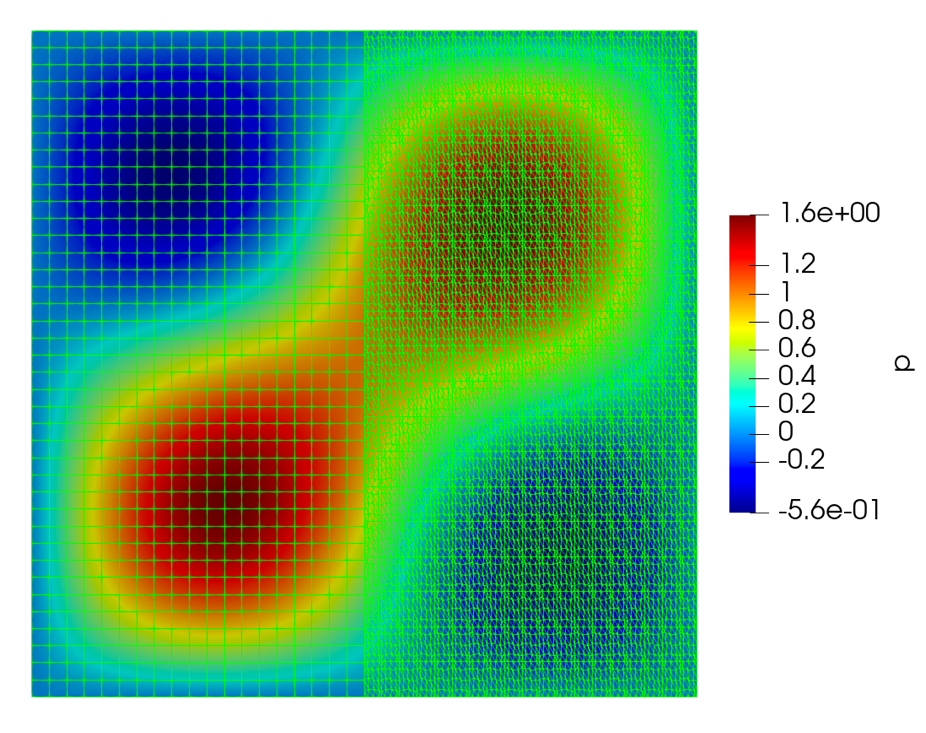
\includegraphics[width=0.8\linewidth,trim=4 4 4 4,clip]{figures/split_domain_wave.png}
\caption{Pressure initial condition for test problem, also showing split-domain
	 discretization.}
\label{fig:split_domain}
\end{figure}

Our success metrics for this test problem include
\begin{itemize}
\item{Demonstrating accurate recreation of the total energy of the system, as observed in the numerical simulation of the problem, via a total energy relation derived from the
spatial and interfacial schema.}
\item{Demonstrating that this energy does not increase (condition for semi-discrete stability).}
\item{Demonstrating the prescribed order of accuracy using L2 norms.}
\end{itemize}

Upon fulfillment of these goals, extension to three dimensions will be considered.

%===========================================================================
\subsection{Results}
(Insert text here)

%===========================================================================
\subsection{Outlook}

\subsubsection{Current Status}

\subsubsection{Risk Mitigation}

%===========================================================================
